Как было рассмотрено ранее, наличие электрического поля, приложенного
к пьезоэлектрическому кристаллу, вызывает изменение межплоскостного расстояния.
Таким образом, был измерен сдвиг рефлексов (рис. \ref{ris:d11_experiment}), и на основании выражения
 (см. \ref{eq:piezomodule_l}) был рассчитан модуль d11 для кристалла LGT.

\begin{figure}[H]
  \centering
  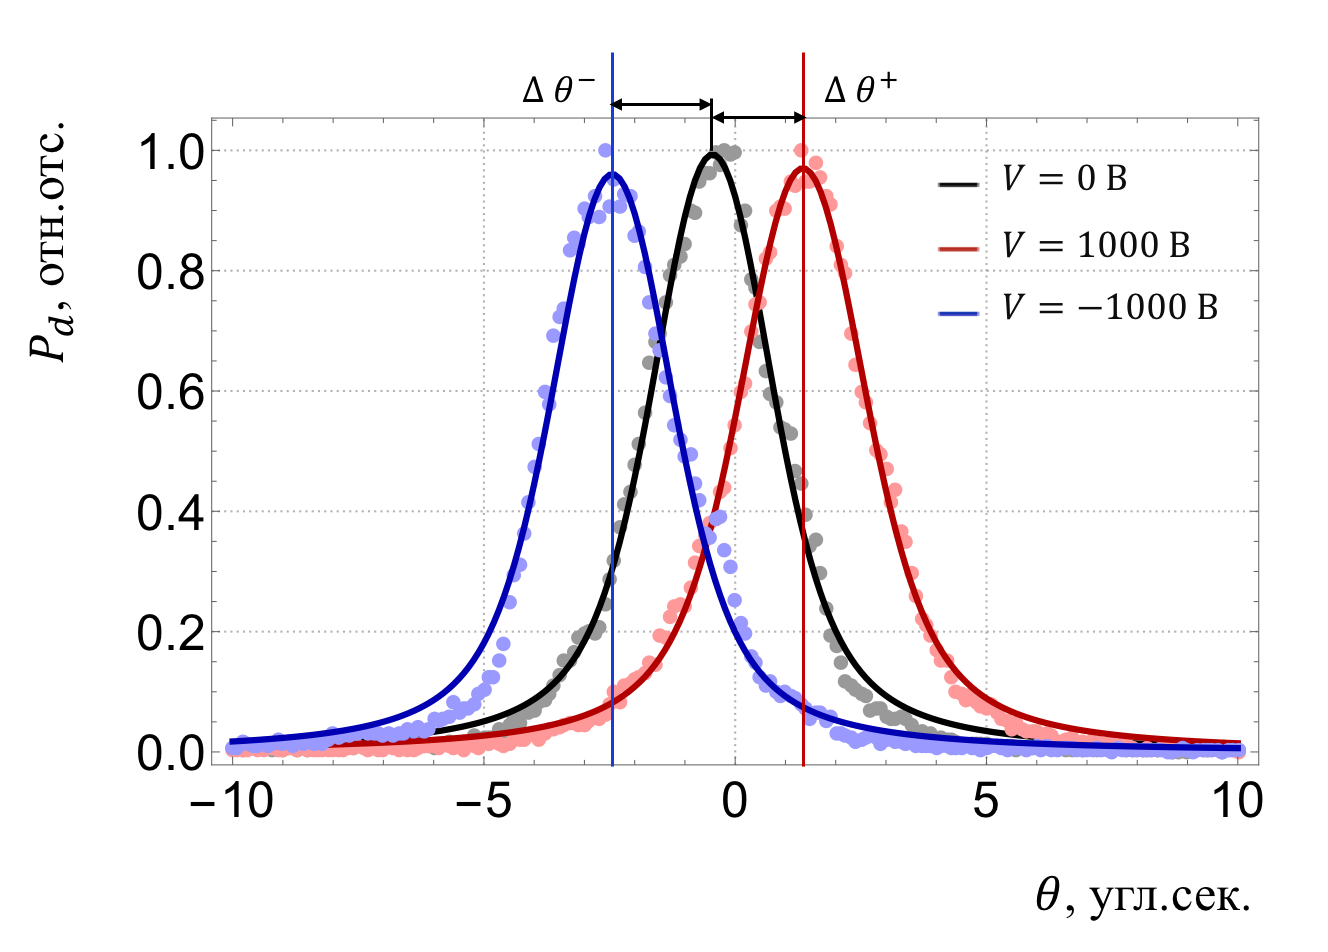
\includegraphics[width=0.7\textwidth]{images/peak_shift_1000v.png}
  \caption{Наблюдаемый сдвиг двухкристальной КДО (эксперимент). Кристалл-монохроматор: Si(440)
  кристалл-образец: LGT(440), толщина кристалла $l = 0.27мм$ }
  \label{ris:d11_experiment}
\end{figure}

Экспериментальное изменение брэгговского угла имеет величину равную 1.89 угл.сек., таким образом
наблюдается хорошее соответствие измеренного пьезомодуля $d11 = (6.8 \pm 0.3 ) 10^{-12}$ по данным
двухкристальной дифрактометрии с другими, нерентгеновскими методами: $d11 = 6.5 \cdot 10^{-12}$ \cite{LGT_piezo_d11}.
Погрешность для данного метода, рассчитывалась исходя из погрешности
аппроксимации, погрешности определения образца и приложенного к нему поля.
В перспективе планируется восстановиться матрицу пьезомодулей с помощью
ренгенодифракционного метода полностью, решая систему уравнений полученную из рассуждений
приведенных в пункте (\ref{sec:pieao_method}).
